\documentclass[10pt,a4paper]{article}

\usepackage[italian]{babel}
\usepackage{amsmath}
\usepackage{amsfonts}
\usepackage{amssymb}

\usepackage[left=1cm,right=1cm,top=1cm,bottom=2cm]{geometry}

\usepackage{txfonts}
\usepackage[T1]{fontenc}

%\usepackage{blindtext}
%\usepackage[T1]{fontenc}
\usepackage[utf8]{inputenc}

\usepackage{titlesec}
\setcounter{secnumdepth}{4}
\titleformat{\paragraph}{\normalfont\normalsize\bfseries}{\theparagraph}{1em}{}
\titlespacing*{\paragraph}{0pt}{3.25ex plus 1ex minus .2ex}{1.5ex plus .2ex}

\usepackage{graphicx}
\usepackage{subcaption}

\usepackage{wrapfig}

\pagenumbering{arabic}
\pagestyle{plain}

\begin{document}


\subsection{L'imu}

L'imu (inertial measurement unit) serve a misurare le forze ad esso applicate e l'orientazione dello stesso. Questo viene solitamente fatto combinando i dati di accelerometro, magnetometro e giroscopio. In particolare l'accelerometro misura le accelerazioni, da cui in condizioni di moto inerziale si pu\`o estrarre il vettore gravit\`a sui 3 assi determinando quindi l'angolazione rispetto al suolo. Il magnetometro rileva invece il campo magnetico terrestre su 3 assi, dando cos\`i indicazione della direzione "nord". Infine il giroscopio restituisce le accelerazioni angolari.
Per questo specifico progetto si sono utilizzati i moduli commerciali "MPU-6050" e "HMC5883L", rispettivamente come accelerometro pi\`u giroscopio e magnetometro. 

\begin{figure}[h]
    \centering
    \begin{subfigure}[b]{0.3\textwidth}
        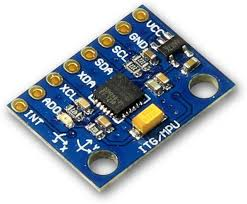
\includegraphics[height=0.75\textwidth]{MPU-6050.jpg}
        \caption{A white penis}
        \label{fig:gull}
    \end{subfigure} 
    \begin{subfigure}[b]{0.3\textwidth}
        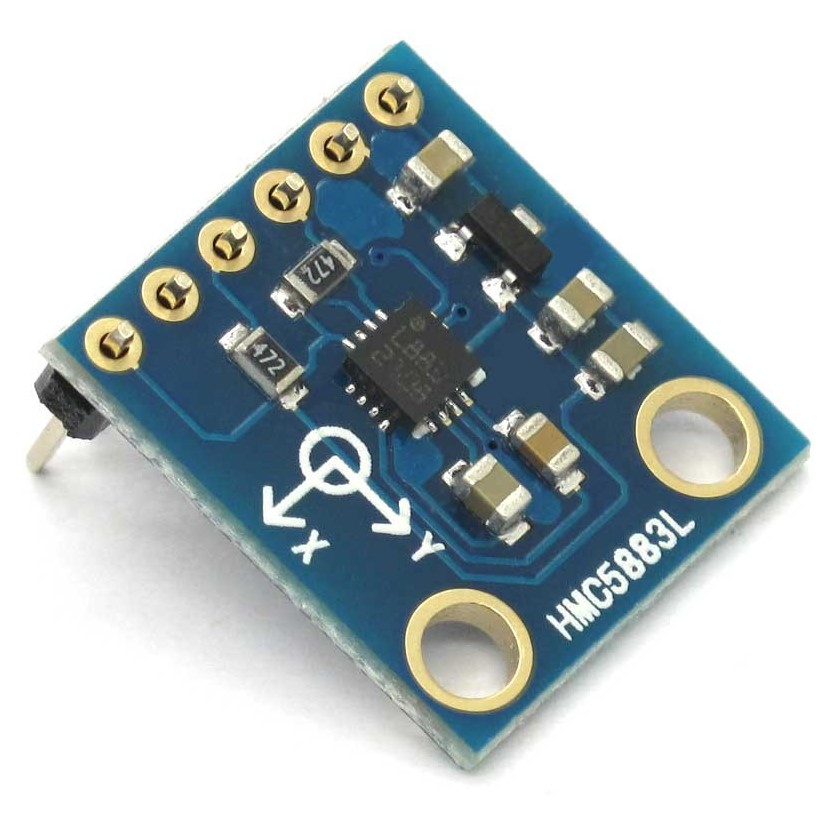
\includegraphics[height=0.75\textwidth]{HMC5883L.jpg}
        \caption{A black penis}
        \label{fig:tiger}
    \end{subfigure}
    \caption{Pictures of penis}\label{fig:animals}
\end{figure}




\end{document}